\documentclass[]{minimal}
\usepackage{tikz}
\usetikzlibrary{arrows.meta}

\begin{document}
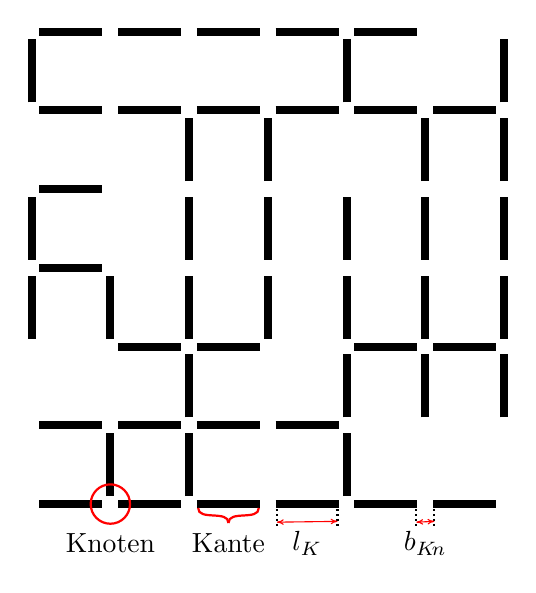
\begin{tikzpicture}

\foreach \x/\y in {0/0, 1/0, 2/0, 3/0, 4/0, 5/0, 0/1, 1/1, 2/1, 3/1, 1/2, 2/2, 4/2, 5/2, 0/3, 0/4, 0/5, 1/5, 2/5, 3/5, 4/5, 5/5, 0/6, 1/6, 2/6, 3/6, 4/6}  
	\draw[shorten >= .1cm, shorten <= .1cm, line width=.1cm] (\x,\y) -- (\x+1,\y);
\foreach \x/\y in {1/0, 2/0, 4/0, 2/1, 4/1, 5/1, 6/1, 0/2, 1/2, 2/2, 3/2, 4/2 ,5/2, 6/2, 0/3 ,2/3, 3/3, 4/3, 5/3, 6/3, 2/4, 3/4,  5/4, 6/4, 0/5, 4/5, 6/5}  
	\draw[shorten >= .1cm, shorten <= .1cm, line width=.1cm] (\x,\y) -- (\x,\y+1);

\draw[red, thick] (1,0) circle[radius=.25cm];
\draw[red, thick] (2.115,-.05) to [out=270, in=90] (2.5,-.24);
\draw[red, thick] (2.885,-.05) to [out=270, in=90] (2.5,-.24);
\begin{scope}[densely dotted, thick]
\draw (4.885,0) -- (4.885,-.3);
\draw (5.115,0) -- (5.115,-.3);
\draw (3.115,0) -- (3.115,-.3);
\draw (3.885,0) -- (3.885,-.3);
\end{scope}
\begin{scope}[red, thin, {<[width=2]}-{>[width=2]}]
\draw (4.885,-.23) -- (5.115,-.22);
\draw (3.115,-.23) -- (3.885,-.22);
\end{scope}

\draw (1,-.5) node {Knoten};
\draw (2.5,-.5) node {Kante};
\draw (3.5,-.5) node {$l_K$};
\draw (5,-.5) node {$b_{K\hspace{-1.5pt} n}$};

\end{tikzpicture}
\end{document}